\begin{appendix}

\chapter{Implementation}\label{ap:a}

Our method is written in C++17 and uses the most recent version of
FALCONN\footnote{\url{https://falconn-lib.org/}} and
Eigen\footnote{\url{https://eigen.tuxfamily.org}} 3.3.4.

The input must be a CSV (i.e. comma-separated) file and may or may not have a header
consisting of alphanumeric column names. The following listing shows the helptext
of the program and lists the default parameters.

\begin{lstlisting}[breaklines,postbreak=\mbox{\textcolor{red}{$\hookrightarrow$}\space}, basicstyle=\ttfamily,caption={Helptext of our implementation}]
usage: ./ktsne opts FILE
where opt in opts is one of the following:

  -p                       ... perplexity (effective number of neighbors per point). tunable parameter, default = 30
  -n                       ... stepsize eta of gradient descent, default = 200
  -x, --early-exaggeration ... early exaggeration value, default = 12
  -X, --late-exaggeration  ... late exaggeration value, default = 12
  -i, --max-iter           ... number of gradient descent iterations, default = 1000
  -s, --seed               ... random seed

  -k, --k-lo ... lower bound for k-means k, default = 30
  -K, --k-hi ... upper bound for k-means k, default = 30

  --random-init ... initialize using a Gaussian distribution with stddev 10e-4
  --pca-init    ... initialize with PCA

  --num-hash-tables ... number of hash tables for FALCONN lsh. tunable parameter, default = 100
  --num-hash-bits   ... number of hash bits, controls number of buckets per table. automatically set to max(16, log2(n)) if -1 is passed, default = -1
  --num-probes      ... number of probes for multi-probe LSH. tunable parameter (inverse relation to L), default = -1

  --[no-]compute-objective  ... compute objective in every iteration, default = off
  --[no-]print-intermediate ... print intermediate embedding to file every iteration (for creating GIFs), default = off

  --use-hyperplane          ... use hyperplane LSH (instead of cross-polytope), default = off
  --use-cross-polytope      ... use cross-polytope LSH (instead of hyperplane LSH), default = on

  -h ... this message

and FILE is a csv file.

ktsne is an accelerated approximative version of tsne which uses LSH and kmeans in its computation.
\end{lstlisting}

Upon starting, the program prints an overview of all parameter settings and then prints the
iteration number every 100 iterations to communicate progress. Per default, the objective is
not printed because its computation is tedious and the approximated objective is not very meaningful
(see Chapter~\ref{ch:eval}).

\chapter{Squared Distance Computation Performance Experiment}\label{ap:b}

An important part of the computation of the gradient in our method, as well as
all other variants of $t$-SNE, are the pairwise squared Euclidean distances between
all points in the low-dimensional space. We attempted to optimize this process
and compared three different approaches using Eigen. The first is a na\"ive implementation:

\begin{lstlisting}[breaklines,postbreak=\mbox{\textcolor{red}{$\hookrightarrow$}\space}, basicstyle=\ttfamily,caption={Na\"ive approach}]
    Eigen::MatrixXd D(X.rows(), Y.rows());
    for(size_t i = 0; i < X.rows(); ++i) {
        for(size_t j = 0; j < Y.rows(); ++j) {
            D(i, j) = (X.row(i) - Y.row(j)).squaredNorm();
        }
    }
\end{lstlisting}

This approach explicitly computes all $n \times m$ pairs. The second approach uses Eigen's
internal iteration mechanism by making use of \texttt{rowwise}, but still uses external iteration.
Using internal iteration should result in a speedup due to optimizations internal to Eigen.

\begin{lstlisting}[breaklines,postbreak=\mbox{\textcolor{red}{$\hookrightarrow$}\space}, basicstyle=\ttfamily,caption={Rowwise approach}]
    Eigen::MatrixXd D(X.rows(), Y.rows());
    for (int i = 0; i < Y.rows(); i++)
        D.col(i) = (X.rowwise() - Y.row(i)).rowwise().squaredNorm().transpose();
\end{lstlisting}

The third variant only uses internal iteration and is the most complex. We applied the binomial
theorem $(a - b)^2 = a^2 - 2ab + b^2$. This has the presumptive advantage that we can offload
a lot of the computational effort onto Eigen's matrix-matrix multiplication, which should result
into a considerable speedup.

\begin{lstlisting}[breaklines,postbreak=\mbox{\textcolor{red}{$\hookrightarrow$}\space}, basicstyle=\ttfamily,caption={Binomial theorem approach}]
    Eigen::MatrixXd D(X.rows(), Y.rows());
    D = ((X * Y.transpose() * -2).colwise() + X.rowwise().squaredNorm()).rowwise() + Y.rowwise().squaredNorm().transpose();
\end{lstlisting}

\begin{figure}[tbp]
    \centering
    \includegraphics[width=\textwidth]{img/matmult_benchmark}
    \caption{Comparison in runtime between 3 approaches to computing all-pairs squared Euclidean distances}
    \label{fig:matmult}
\end{figure}

Figure~\ref{fig:matmult} shows the runtime comparison between the three aforementioned
approaches. We ran 10 repeats for every problem size $n$. The matrices $X$ and $Y$
were of dimensions $n \times 2$ and $50 \times 2$, which corresponds to the use case
in our method. It shows that the third variant performs well and the gaps between the methods
keep widening as $n$ increases. We thus used the binomial form in our implementation.

\chapter{Selected Embedding Comparison}\label{ap:c}

On the next pages, we present the embeddings of 6 selected datasets---cifar, com-amazon,
fashion MNIST, pubmed, hollywood and wiki-topcats---found by the 4 methods compared in
our work.

As can be seen, our method tends to compute embeddings that appear somewhat distorted
and not as spherical especially when compared to FI$t$-SNE and Barnes-Hut $t$-SNE.
This may be due to the large exaggeration values used or due to the approximation error.
It is notable, though, that the distortion is also present in UMAP's embeddings. Overall,
all embeddings appear sensible. Do note that the labels for com-amazon and wiki-topcats
were generated using graph clustering and indeed match the embeddings well.

\begin{figure}[tbp]
  \centering
  \begin{subfigure}{0.45\linewidth}
    \centering
    \includegraphics[width=\linewidth]{img/emb/bhtsne_cifar}
    \caption{Barnes-Hut $t$-SNE}
  \end{subfigure}
\begin{subfigure}{0.45\linewidth}
  \centering
    \includegraphics[width=\linewidth]{img/emb/fitsne_cifar}
    \caption{FI$t$-SNE}
\end{subfigure}
\par\bigskip
\begin{subfigure}{0.45\linewidth}
  \centering
    \includegraphics[width=\linewidth]{img/emb/ktsne_cifar}
    \caption{$kt$-SNE}
\end{subfigure}
  \begin{subfigure}{0.45\linewidth}
    \centering
    \includegraphics[width=\linewidth]{img/emb/umap_cifar}
    \caption{UMAP}
  \end{subfigure}
  \caption{CIFAR}
\end{figure}

\begin{figure}[tbp]
  \centering
  \begin{subfigure}{0.45\linewidth}
    \centering
    \includegraphics[width=\linewidth]{img/emb/bhtsne_com-amazon}
    \caption{Barnes-Hut $t$-SNE}
  \end{subfigure}
\begin{subfigure}{0.45\linewidth}
  \centering
    \includegraphics[width=\linewidth]{img/emb/fitsne_com-amazon}
    \caption{FI$t$-SNE}
\end{subfigure}
\par\bigskip
\begin{subfigure}{0.45\linewidth}
  \centering
    \includegraphics[width=\linewidth]{img/emb/ktsne_com-amazon}
    \caption{$kt$-SNE}
\end{subfigure}
  \begin{subfigure}{0.45\linewidth}
    \centering
    \includegraphics[width=\linewidth]{img/emb/umap_com-amazon}
    \caption{UMAP}
  \end{subfigure}
  \caption{com-amazon}
\end{figure}

\begin{figure}[tbp]
  \centering
  \begin{subfigure}{0.45\linewidth}
    \centering
    \includegraphics[width=\linewidth]{img/emb/bhtsne_fashion_mnist}
    \caption{Barnes-Hut $t$-SNE}
  \end{subfigure}
\begin{subfigure}{0.45\linewidth}
  \centering
    \includegraphics[width=\linewidth]{img/emb/fitsne_fashion_mnist}
    \caption{FI$t$-SNE}
\end{subfigure}
\par\bigskip
\begin{subfigure}{0.45\linewidth}
  \centering
    \includegraphics[width=\linewidth]{img/emb/ktsne_fashion_mnist}
    \caption{$kt$-SNE}
\end{subfigure}
  \begin{subfigure}{0.45\linewidth}
    \centering
    \includegraphics[width=\linewidth]{img/emb/umap_fashion_mnist}
    \caption{UMAP}
  \end{subfigure}
  \caption{Fashion MNIST}
\end{figure}

\begin{figure}[tbp]
  \centering
  \begin{subfigure}{0.45\linewidth}
    \centering
    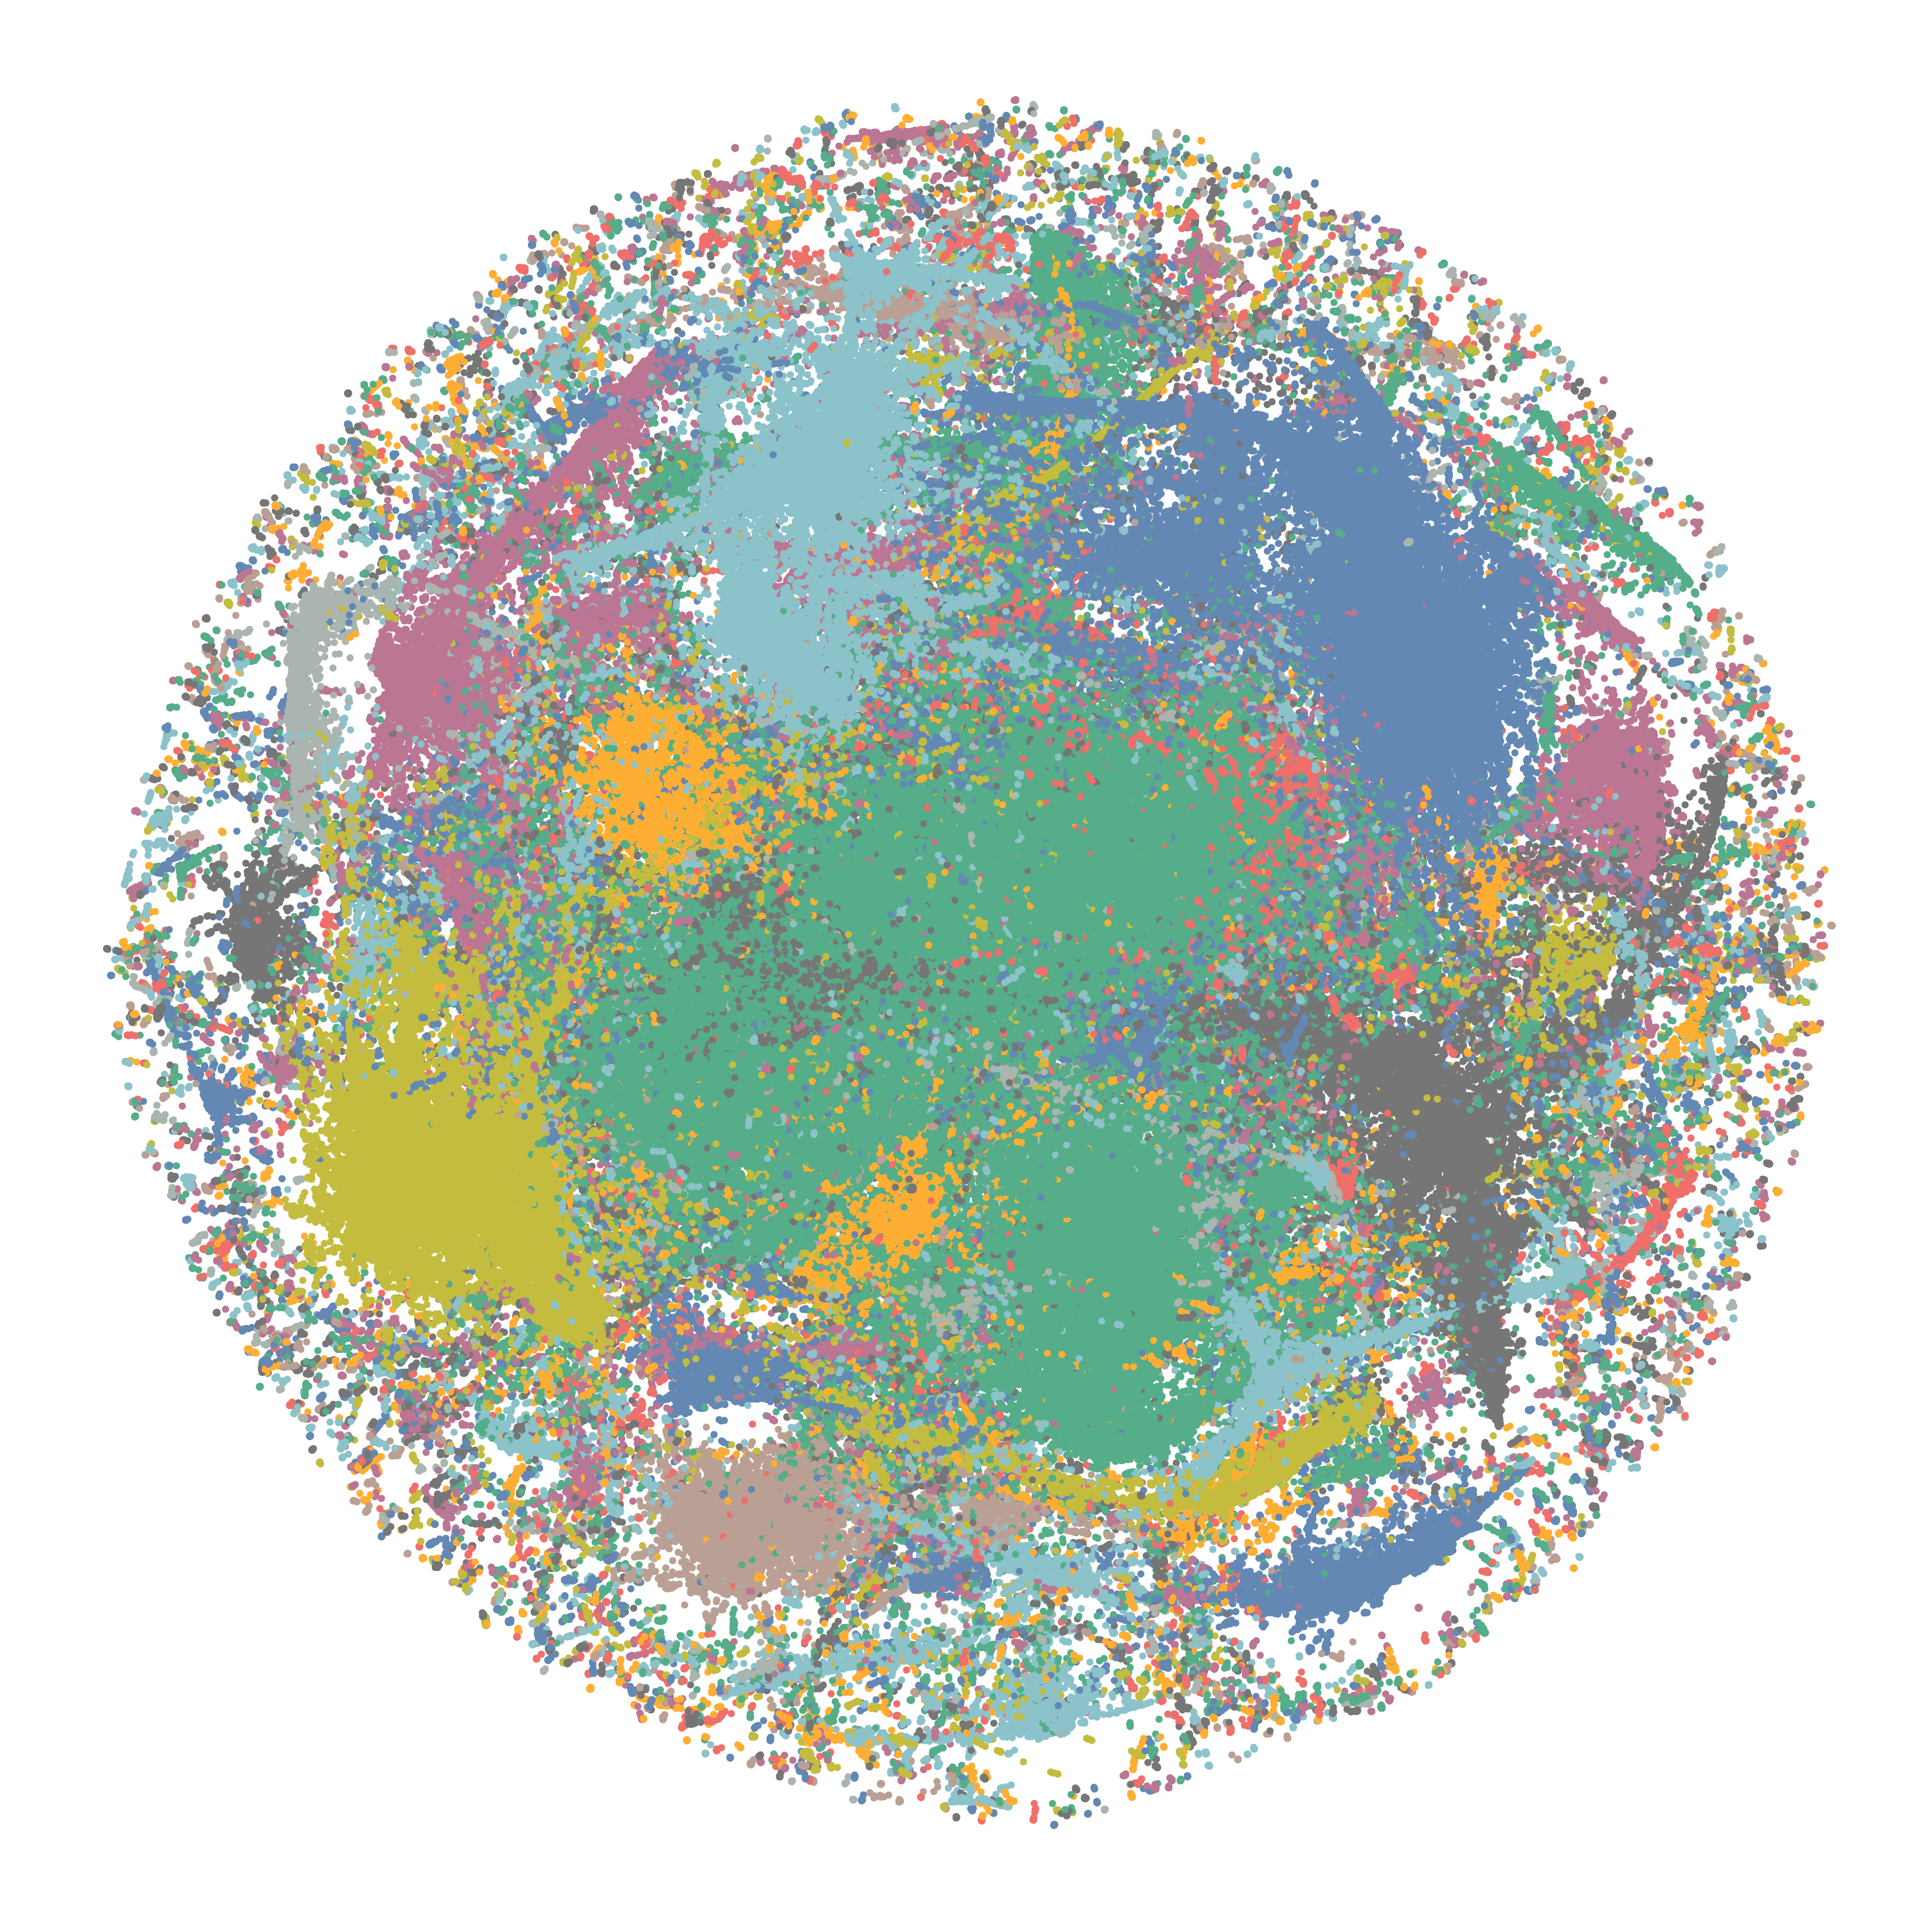
\includegraphics[width=\linewidth]{img/emb/bhtsne_hollywood}
    \caption{Barnes-Hut $t$-SNE}
  \end{subfigure}
\begin{subfigure}{0.45\linewidth}
  \centering
    \includegraphics[width=\linewidth]{img/emb/fitsne_hollywood}
    \caption{FI$t$-SNE}
\end{subfigure}
\par\bigskip
\begin{subfigure}{0.45\linewidth}
  \centering
    \includegraphics[width=\linewidth]{img/emb/ktsne_hollywood}
    \caption{$kt$-SNE}
\end{subfigure}
  \begin{subfigure}{0.45\linewidth}
    \centering
    \includegraphics[width=\linewidth]{img/emb/umap_hollywood}
    \caption{UMAP}
  \end{subfigure}
  \caption{hollywood}
\end{figure}

\begin{figure}[tbp]
  \centering
  \begin{subfigure}{0.45\linewidth}
    \centering
    \includegraphics[width=\linewidth]{img/emb/bhtsne_pubmed}
    \caption{Barnes-Hut $t$-SNE}
  \end{subfigure}
\begin{subfigure}{0.45\linewidth}
  \centering
    \includegraphics[width=\linewidth]{img/emb/fitsne_pubmed}
    \caption{FI$t$-SNE}
\end{subfigure}
\par\bigskip
\begin{subfigure}{0.45\linewidth}
  \centering
    \includegraphics[width=\linewidth]{img/emb/ktsne_pubmed}
    \caption{$kt$-SNE}
\end{subfigure}
  \begin{subfigure}{0.45\linewidth}
    \centering
    \includegraphics[width=\linewidth]{img/emb/umap_pubmed}
    \caption{UMAP}
  \end{subfigure}
  \caption{pubmed}
\end{figure}

\begin{figure}[tbp]
  \centering
  \begin{subfigure}{0.45\linewidth}
    \centering
    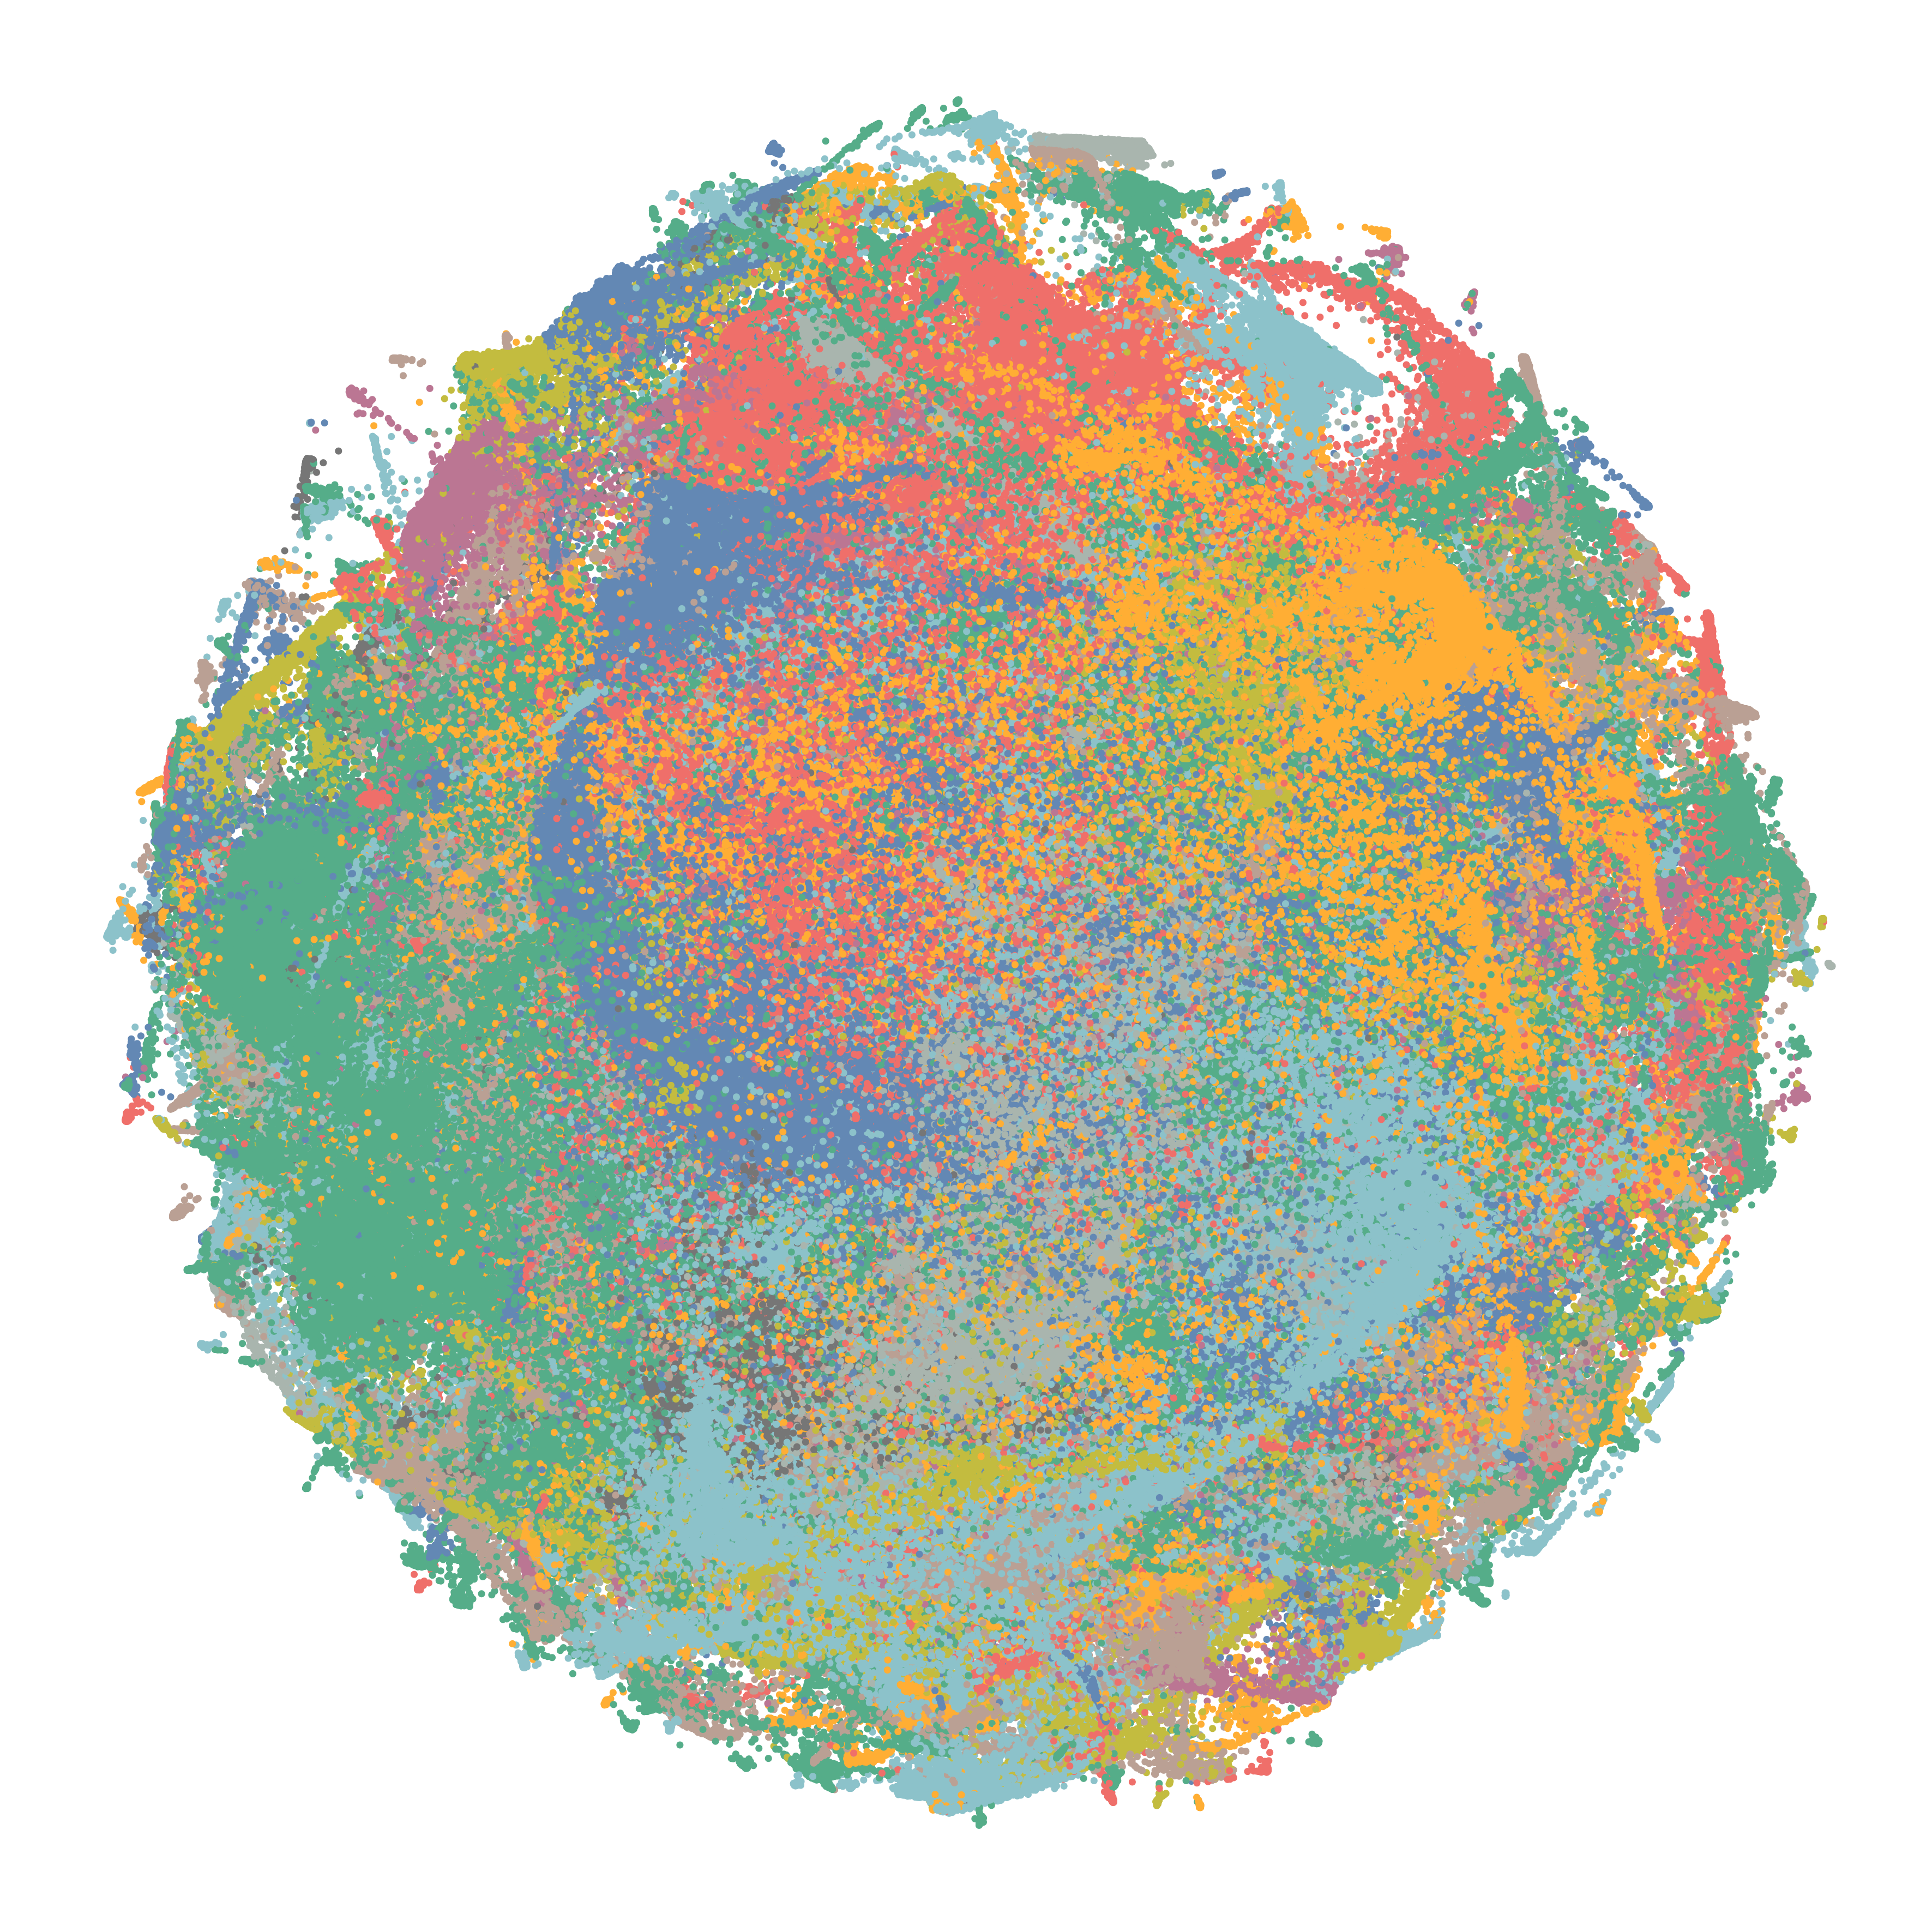
\includegraphics[width=\linewidth]{img/emb/bhtsne_wiki-topcats}
    \caption{Barnes-Hut $t$-SNE}
  \end{subfigure}
\begin{subfigure}{0.45\linewidth}
  \centering
    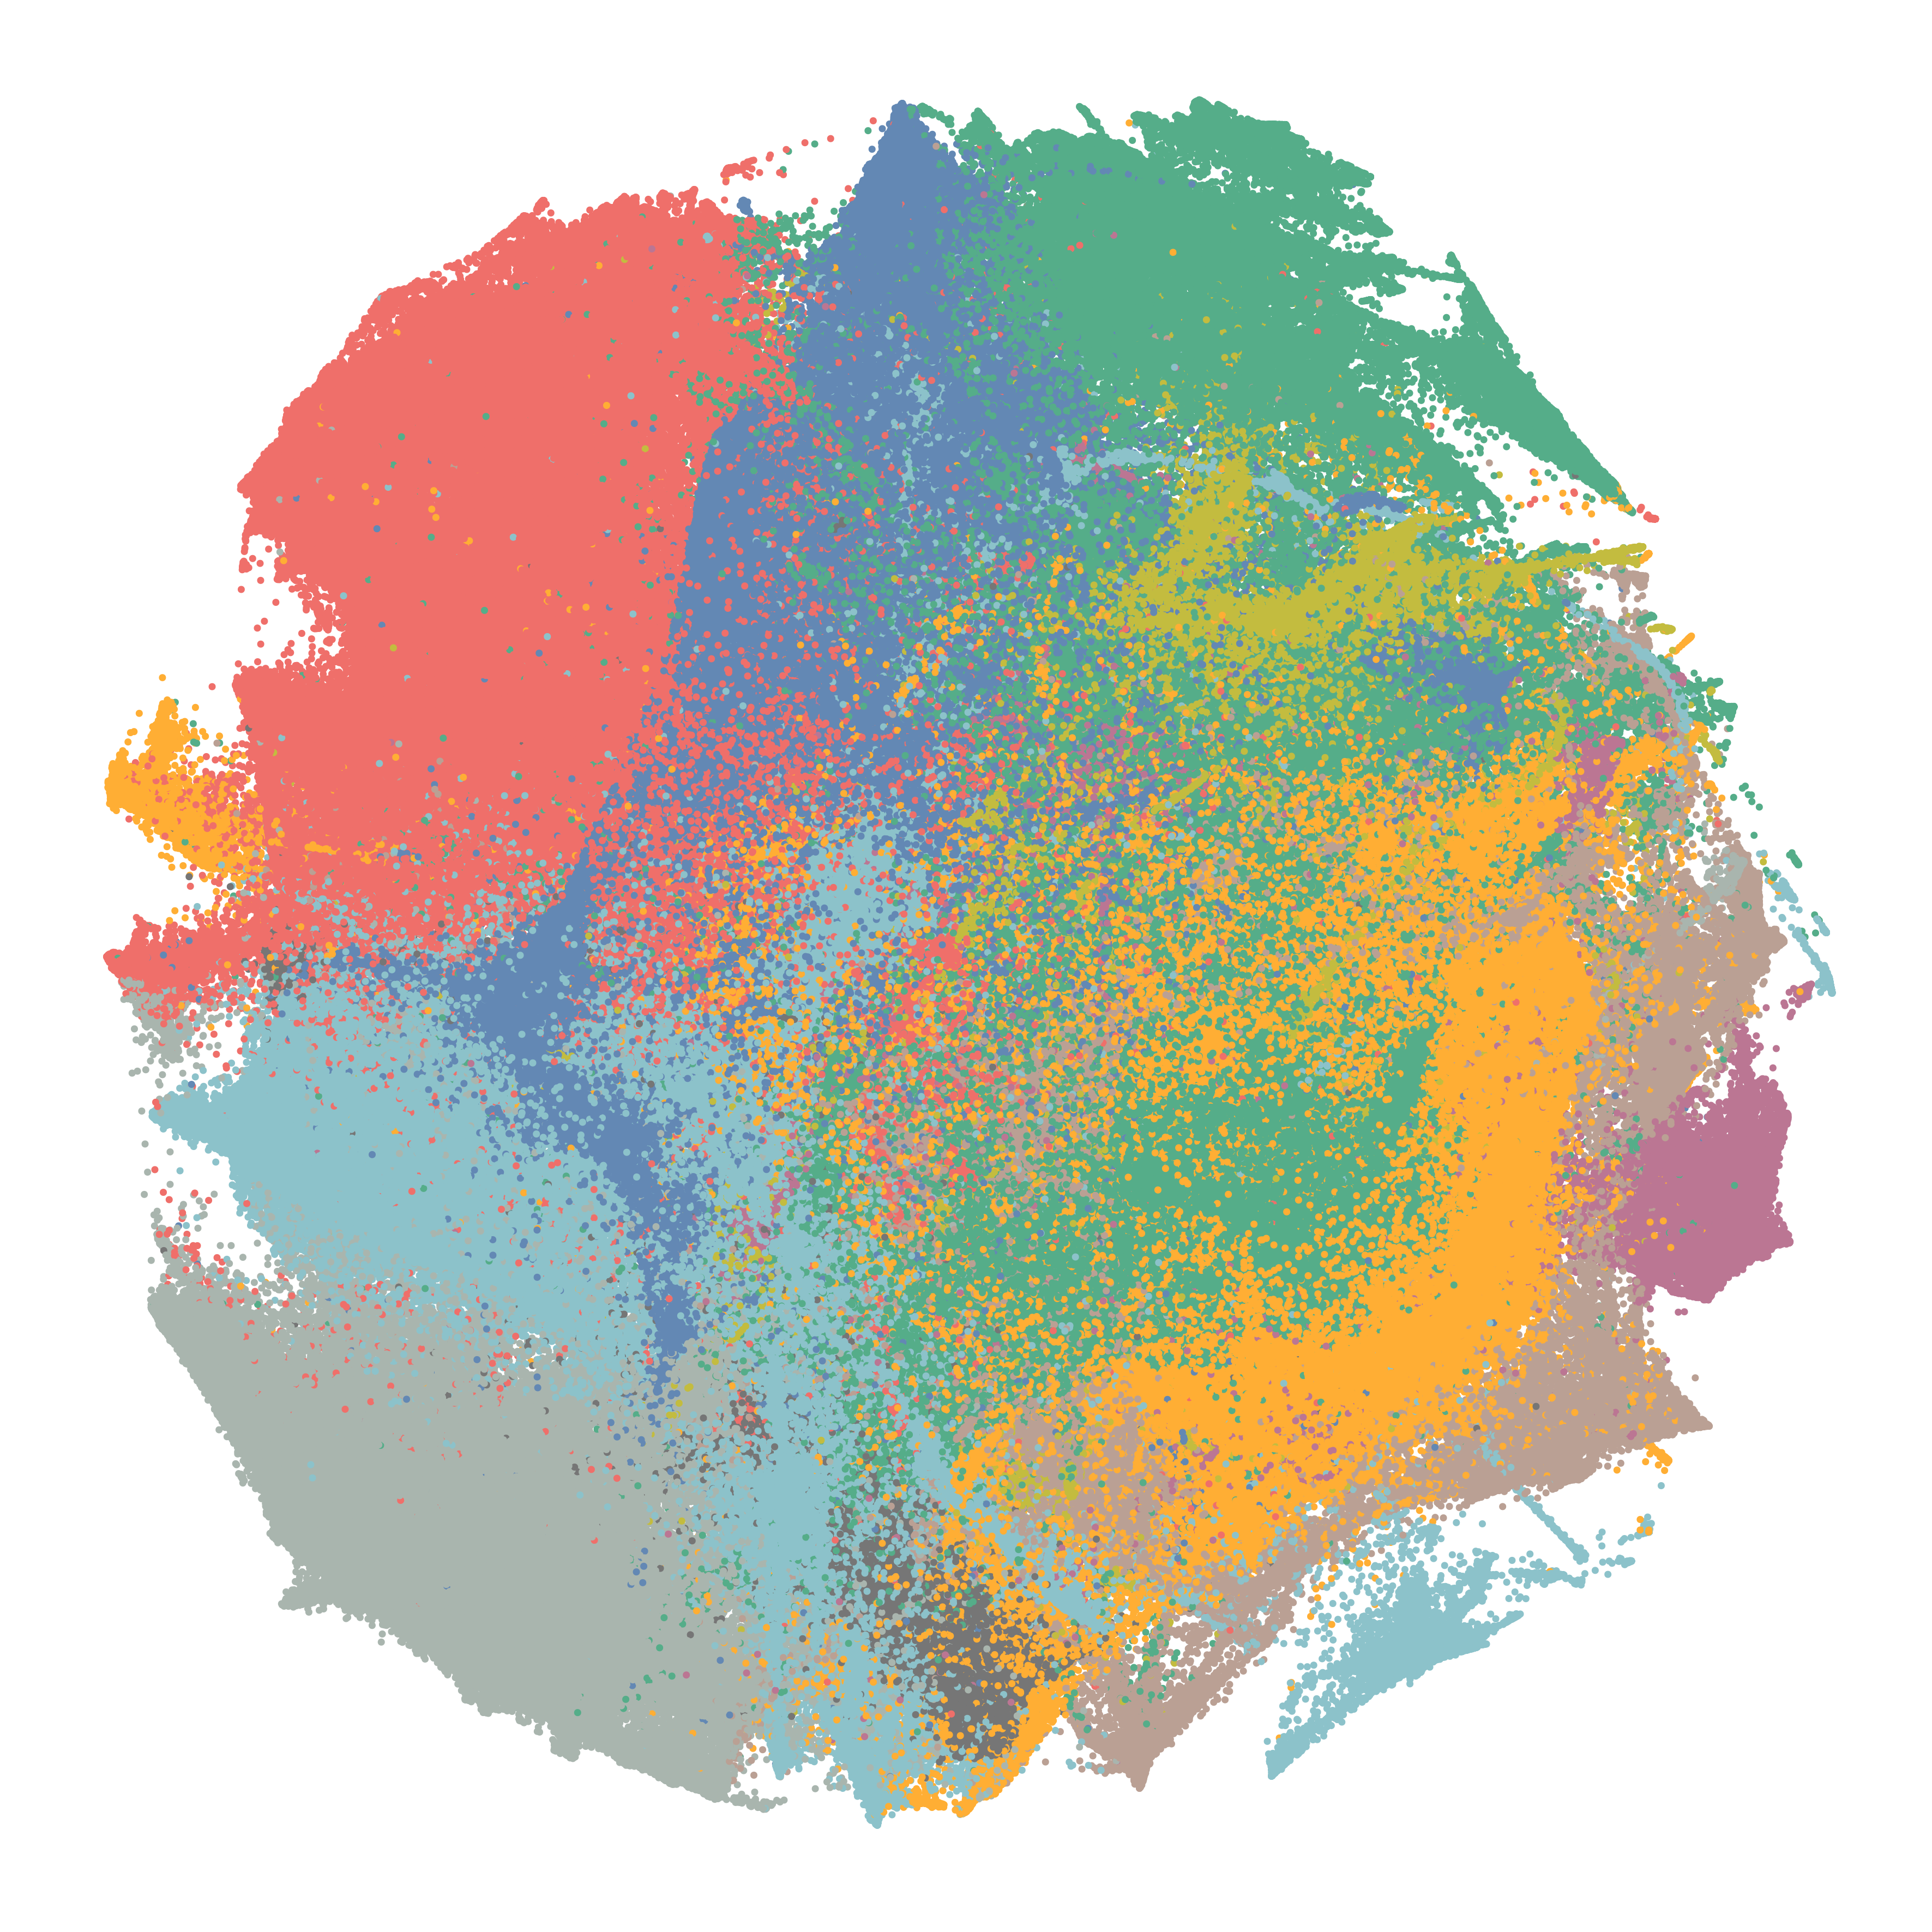
\includegraphics[width=\linewidth]{img/emb/fitsne_wiki-topcats}
    \caption{FI$t$-SNE}
\end{subfigure}
\par\bigskip
\begin{subfigure}{0.45\linewidth}
  \centering
    \includegraphics[width=\linewidth]{img/emb/ktsne_wiki-topcats}
    \caption{$kt$-SNE}
\end{subfigure}
  \begin{subfigure}{0.45\linewidth}
    \centering
    \includegraphics[width=\linewidth]{img/emb/umap_wiki-topcats}
    \caption{UMAP}
  \end{subfigure}
  \caption{wiki-topcats}
\end{figure}

\end{appendix}
